\documentclass[12pt]{book}

\usepackage[utf8]{inputenc}
\usepackage[spanish]{babel}
\parindent = 0cm

\usepackage{amsmath}
\usepackage{amssymb,amsfonts,latexsym,cancel}
\usepackage{graphicx}
\usepackage{float}
\usepackage{subfigure}
\usepackage{vmargin}
\usepackage[usenames,dvipsnames,svgnames,table]{xcolor}

\setpapersize{A4}
\setmargins{2.5cm} % margen izquierdo
{1.5cm}            % margen superior
{16.5cm}           % anchura del texto
{23.42cm}          % altura del texto
{10pt}             % altura de los encabezados
{1cm}              % espacio entre el texto y los encabezados
{0pt}              % altura del pie de página
{2cm}              % espacio entre el texto y el pie de página

\begin{document}

\title{
\begin{center}

\includegraphics[scale=1]{figuras/cartelfiuba.png}\\[3cm]
\end{center}
Circuitos Electrónicos II - 66.10\\ Trabajo Práctico Nº 2\\[2cm]
Análisis del amplificador de potencia del Turner 730\\[1cm]
\begin{flushleft}
Alumnos, Docentes
\end{flushleft}}
\author{}
\date{}
\maketitle
%\tableofcontents

\section{Objetivos}
\subsection{Resumen de objetivos}
ver
\subsection{Desarrollo}
ver

\newpage
\begin{figure}[!ht]
\centering
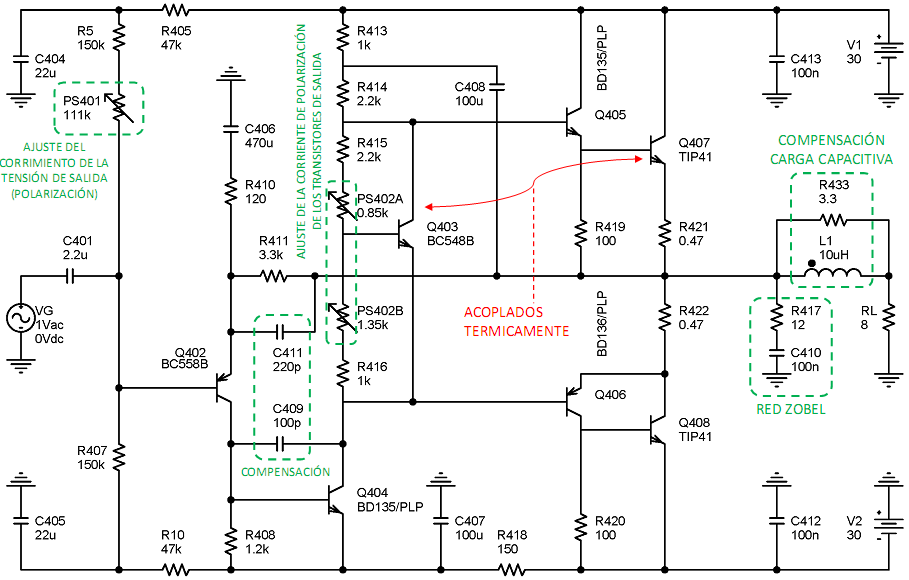
\includegraphics[scale=0.5]{figuras/CircuitoPropuesto.png}
\caption{Circuito a analizar y simular. REEMPLAZAR AGREGANDO ETAPAS}
\label{circuito}
\end{figure}

\newpage
\section{Desarrollo}
\subsection{Punto 1}
\textbf{Enunciado : } Calcular las tensiones de todos los nodos y las corrientes de todas la ramas para VG=0V\\[1cm]
\begin{figure}[H]
\centering
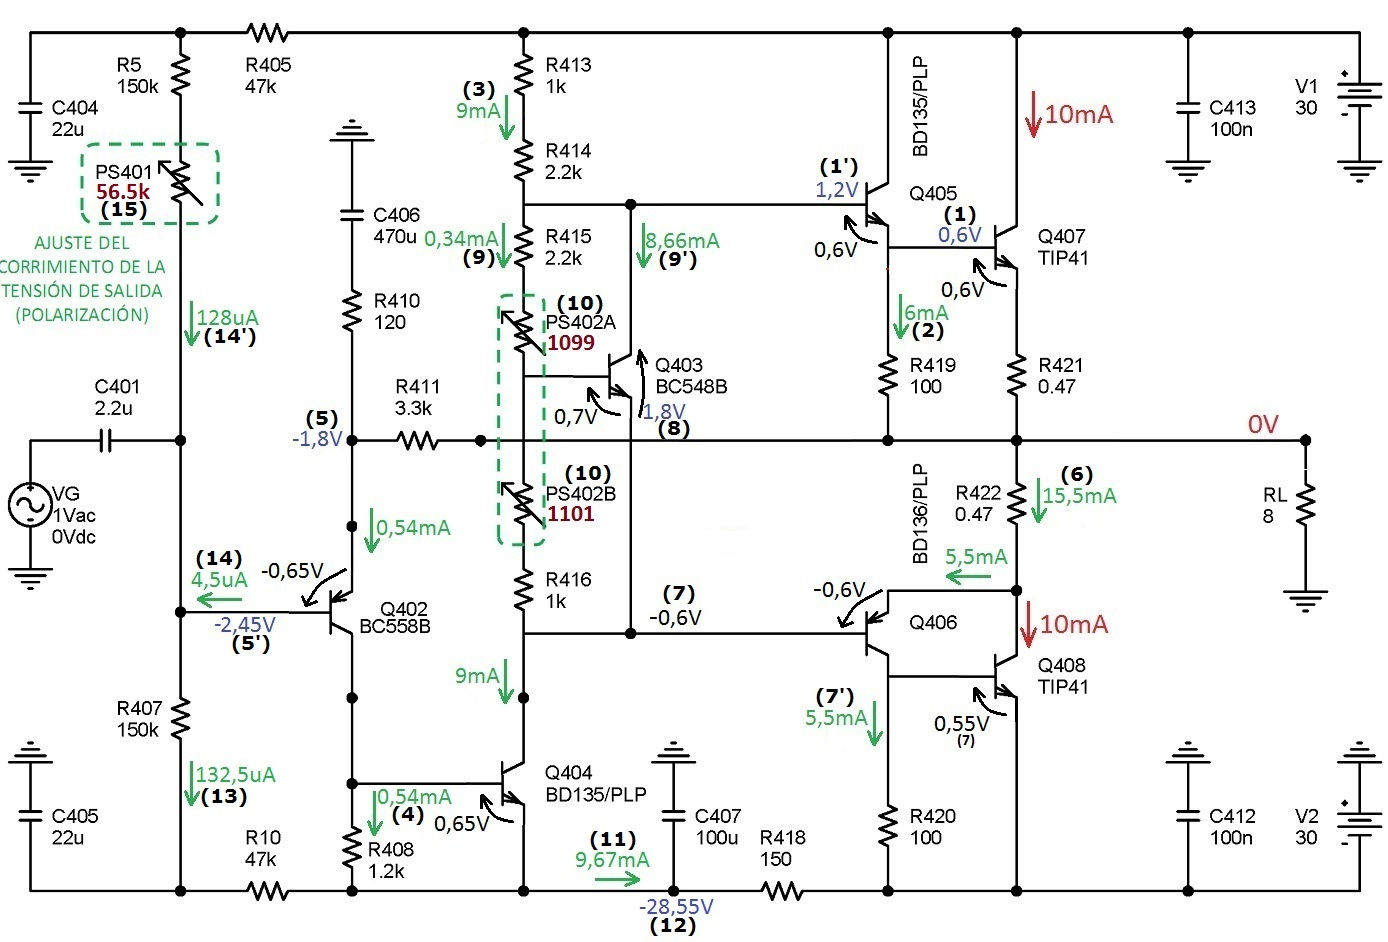
\includegraphics[scale=0.4]{figuras/1-valoresReposo.png}
\caption{Valores de polarización calculados}
\label{figura1}
\end{figure}
Los valores de $\beta$ como los de $V_{BE}$ se tomaron de las hojas de datos de los respectivos transistores, excepto la tensión de Early, $V_{A}$ , que fue tomada del modelo spice correspondiente.
\begin{center}
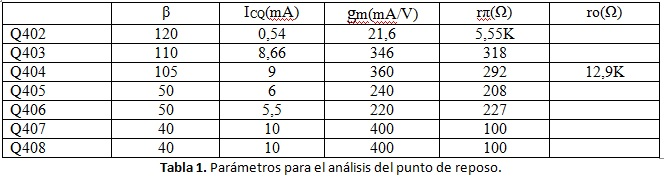
\includegraphics[scale=0.8]{figuras/tabla1.jpg}\\
\end{center}
Se procedió a tomar en cuenta primero los datos de salida $V_{OQ}$=0V e $I_{CQ407/8}$=10mA, se despreciaron todas las corrientes de base de los transistores (excepto $Q_{402}$, para ajustar PS401), con esto se llegó al paso (9). En el paso (10) se aplicó la ecuación del multiplicador de $V_{BE}$  con $V_{CE}$=1,8V, paso (8), obteniéndose:\\
\begin{center}
PS402A=1099$\Omega$  y  PS402B=1101$\Omega$
\end{center}
Luego para los pasos (11) y (12) se propuso que los 9mA de Q404 y los 0,54mA de R408 (9,54mA) pasaran por R418 y y con eso se obtuvo una primer tensión (14) de –28,57V y una corriente en R407 (13) de 132,6$\mu$A, que ajusta levemente a la tensión anterior (14) a –28,55V.\\
Por último (15), para lograr un mejor ajuste de PS401 se tuvo en cuenta la corriente base de $Q_{402}$, obteniéndose :
\begin{center}
PS401=56,5K$\Omega$
\end{center}

\subsection{Punto 2}
\textbf{Enunciado : } Calcular la ganancia de lazo para frecuencias medias (1KHz)\\[1cm]
Para este punto hacemos el esquemático para alterna, reemplazamos la tercera etapa por un bloque con ganancia de tensión unitaria, para mayor claridad.\\
\begin{figure}[H]
\centering
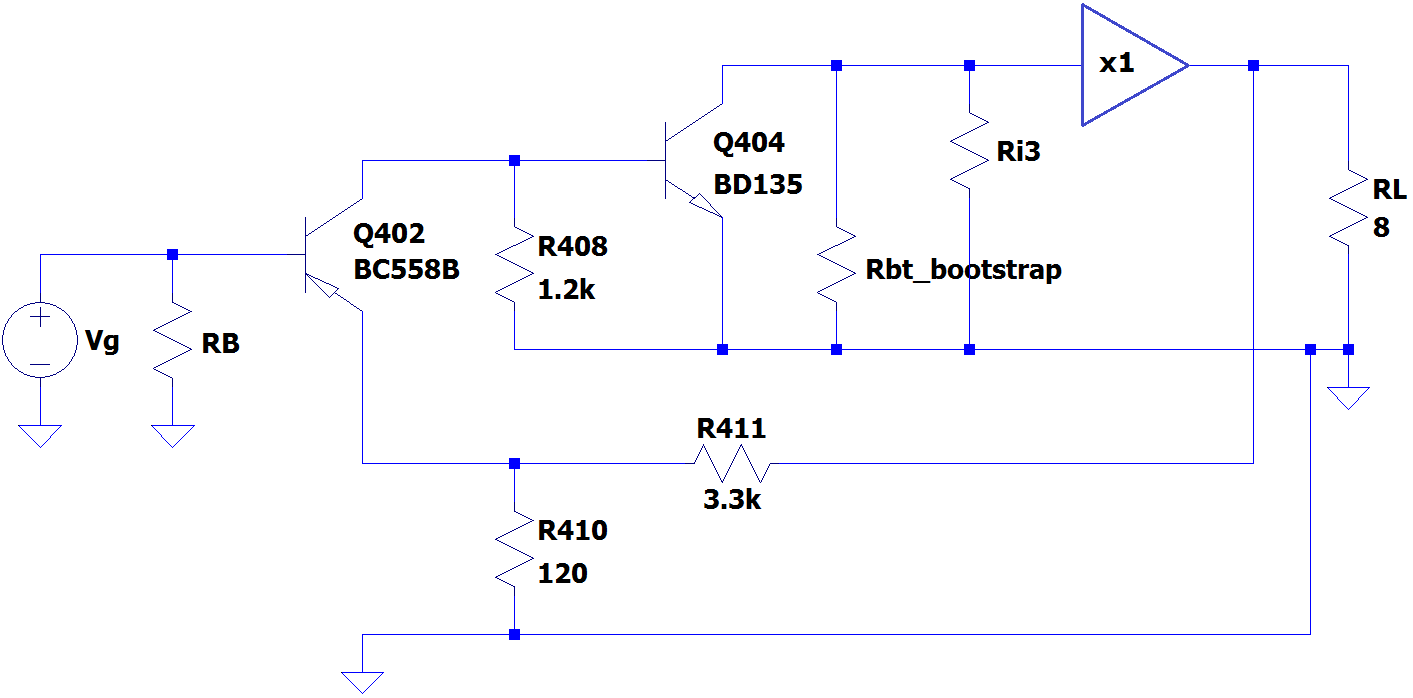
\includegraphics[scale=0.4]{figuras/2-lazoCerrado.png}
\caption{Realimentación Serie-Paralelo}
\label{figura2-1}
\end{figure}
Al muestrear tensión y sumar tensión tenemos que a la entrada se comparte la corriente y a la salida la tensión, entonces parametrizamos la realimentación con parámetros híbridos H.
\begin{center}
El factor de realimentación $f$ , es:\qquad $f$ = $h_{12}$ = $\dfrac{120\Omega}{120\Omega+3,3K\Omega}$ = 0,0135
\end{center}
Luego $h_{11}$=R410//R411 se acopla a la entrada, y $h_{22}$=R410+R411 a la salida para considerar una realimentación ideal:
\begin{figure}[H]
\centering
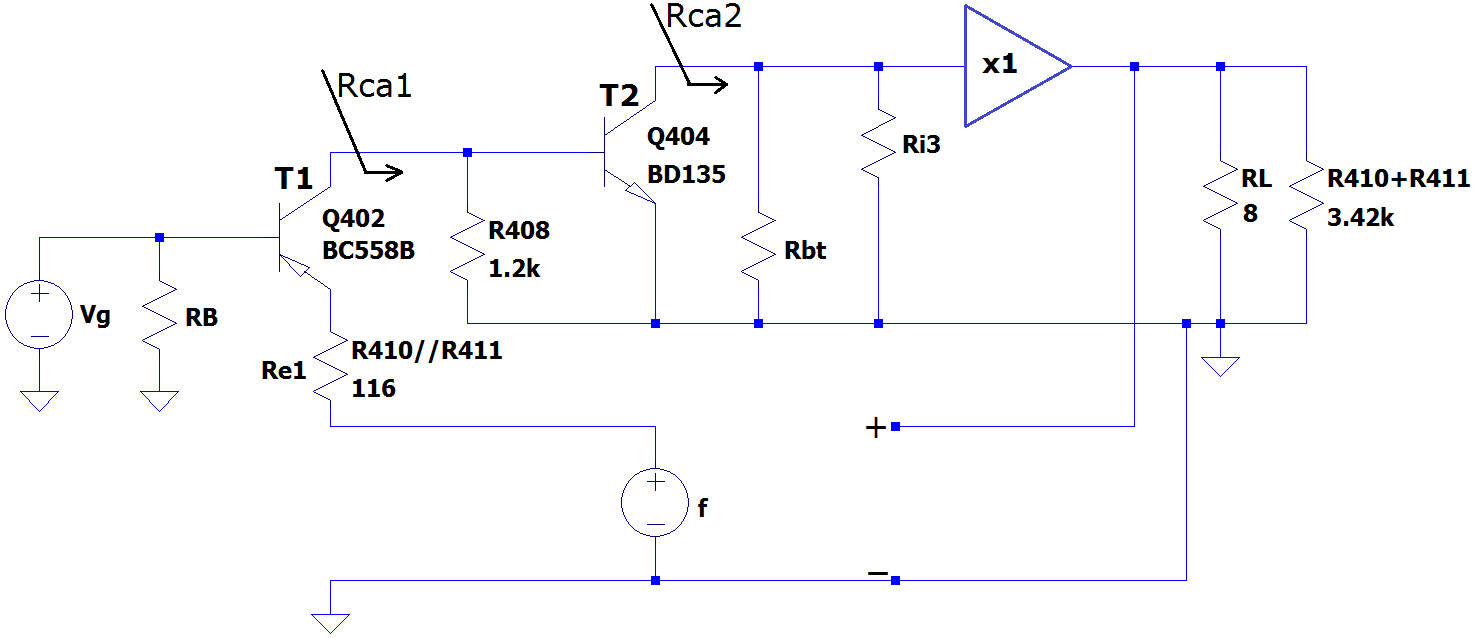
\includegraphics[scale=0.4]{figuras/2-lazoCerradoIdeal.png}
\caption{Realimentación Serie-Paralelo ideal}
\label{figura2-2}
\end{figure}
Se despreció $h_{21}$, el efecto de la salida sobre la entrada.\\[0.5cm]
$Av_{1} = \dfrac{-gm_{1}Rca1}{1+gm_{1} Re1} = \dfrac{-gm_{1}(R408//r_{\pi_2})}{1+gm_{1}(R411//R410)} = -1,45$\\
$Av_{2} = -gm_{2}Rca2 = -gm_{2}(ro_{2}//Ri_{3}//Rbt) = -360\dfrac{mA}{V} 6,9K\Omega = -2484$\\[0.5cm]
Donde :\\
Ri3 $=\beta_{405} \beta_{407} RL = 50$ . 40 . $8\Omega = 16K\Omega$\\
$ro_{2}$ = 12,9K$\Omega$ es la resistencia de salida correspondiente al modelo a $Q_{404}$\\
Rbt = 100 . R414 = 100 . 2,2K$\Omega$ = 220K$\Omega$ es la resistencia de bootstrap
\begin{center}
$\Longrightarrow$   Av = Av1 . Av2 . Av3 = (-1,45)(-2484) 0,99 = 3565,8\\
\end{center}
La ganancia del amplificador a lazo abierto es  $a$ = Av ($\dfrac{zc}{zc+ro}$) ($\dfrac{ri}{zg+ri+Re1}$)\\
Siendo :\\
$zc$ = RL//(R411+R410) = 97,2$\Omega$\\
$ro$ y $ri$ se obtienen mediante simulación: $ro$ = 4$\Omega$ y $ri$ = 38,8K$\Omega$
\begin{center}
$\Longrightarrow$   $a$ = 3414\\
\end{center}
Con lo que la ganancia a lazo abierto, T, es :
\begin{center}
T = $a$ $f$ = 119,5\\
\end{center}

\subsection{Punto 3}
\textbf{Enunciado : } Calcular la ganancia global para frecuencias medias (1KHz)\\
\begin{center}
Ganacia global\quad A = $\dfrac{a}{1+af}$ = 28,3
\end{center}

\subsection{Punto 4}
\textbf{Enunciado : } Calcular la máxima potencia obtenible sobre la carga para frecuencias medias (1KHz)\\[1cm]
Máxima potencia disipada por el transistor $Q_{407/8}$:\quad $Pc_{max}=\dfrac{Vcc^{2}}{\pi^{2}RL}=11,4W$\\[0,75cm]
Que es el 40\% de la máxima potencia disipada en la carga $P_{cargamax}$, entonces :
\begin{center}

\end{center}

\subsection{Punto 5}
\textbf{Enunciado : } Calcular la impedancia de entrada para frecuencias medias (1KHz)\\[1cm]
Ri = [($1+af$) Rib]//Rb\\
Rib = r$\pi_{Q402}$ + $\beta_{Q402}$ (R410//R411) = 19,9K$\Omega$\\
Rb = (R5 + PS401) // R407 = 86,9K$\Omega$
\begin{center}
$\Longrightarrow$  Ri = 86,9K$\Omega$
\end{center}

\subsection{Punto 6}
\textbf{Enunciado : } Calcular la impedancia de salida para frecuencias medias (1KHz)\\[1cm]
Mediante simulación se obtuvo que ro=4$\Omega$\\
Por lo que $Ro=\dfrac{ro}{1+af}$ al estar muestreando tensión.
\begin{center}
$\Longrightarrow$  Ro = 33,2m$\Omega$
\end{center}

\subsection{Punto 7}
\textbf{Enunciado : } Calcular el factor de amortiguamiento para frecuencias medias (1KHz)\\[1cm]

Factor de amortiguamiento, Df (Damping factor) :\qquad $Df=\dfrac{RL}{Ro}$\\
\begin{center}
$\Longrightarrow$  Df = $\dfrac{8\Omega}{33,2m\Omega}$ = 240
\end{center}
Debido a que el cable de conexión entre la carga y el nodo de salida puede aumentar Df, se coloca la red de compensación capacitiva......FALTA

\subsection{Punto 8}
\textbf{Enunciado : } Calcular la máxima tensión pico sobre la carga para frecuencias medias (1KHz)\\[1cm]
Vimos en el punto 4 que :\quad $P_{cargamax}$=28,5W\\[0.25cm]
Entonces\quad $V_{max}$ = 15,1V
\begin{center}
$\Longrightarrow$  $V_{picomax}$ = 21,3V
\end{center}

\subsection{Punto 9}
\textbf{Enunciado : } Calcular la máxima eficiencia obtenible con este amplificador para frecuencias medias (1KHz)\\[1cm]
Eficiencia máxima\quad $\eta_{max}=\dfrac{P_{cargamax}}{P_{fuente}}=\dfrac{\frac{Ip.Vp}{2}}{\frac{2 Ip.Vcc}{\pi}}$
\begin{center}
$\Longrightarrow$  $\eta_{max}$ = 55\%
\end{center}

\subsection{Punto 10}
\textbf{Determinar : }\\

\subsubsection{Punto 10.a)}
\textbf{Enunciado : } El tamaño de los disipadores para cada transistor (resistencia térmica disipador ambiente)\\[1cm]

\subsubsection{Punto 10.b)}
\textbf{Enunciado : } Encontrar el disipador comercial que podría utilizarse para construir un prototipo funcional\\[1cm]

\subsubsection{Punto 10.c)}
\textbf{Enunciado : } Comparar con los disipadores utilizados originalmente por Turner y obtener conclusiones\\[1cm]

\subsection{Punto 11}
\textbf{Simular el comportamiento estático y dinámico del amplificador determinando:}\\

\subsubsection{Punto 11.a)}
\textbf{Enunciado : } Medir las tensiones de todos los nodos y las corrientes de todas las ramas para VG=0V\\[1cm]
\begin{figure}[H]
\centering
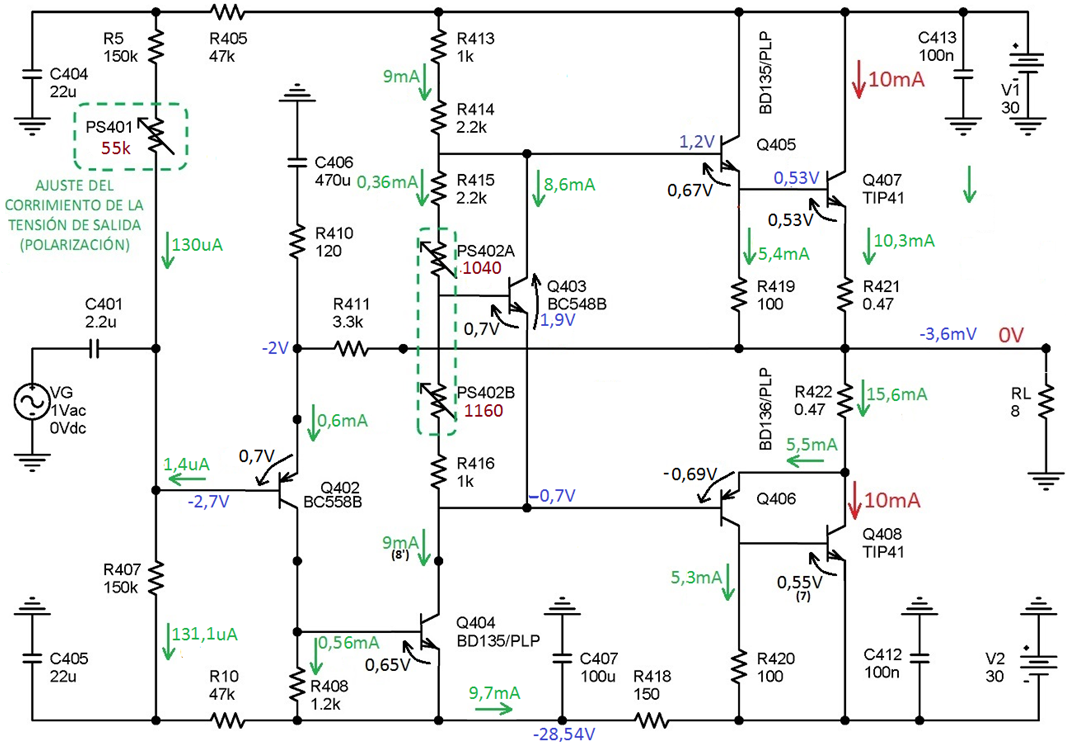
\includegraphics[scale=0.4]{figuras/11-a-valoresReposo.png}
\caption{Valores obtenidos de la simulación del punto de operación}
\label{figura11a}
\end{figure}
Vemos una gran similitud con los valores calculados anteriormente, Fig.\eqref{figura1}

\subsubsection{Punto 11.b)}
\textbf{Enunciado : } Medir la impedancia de entrada en función de la frecuencia (desde 0,1Hz hasta 1GHz)\\[1cm]
\begin{figure}[H]
\centering
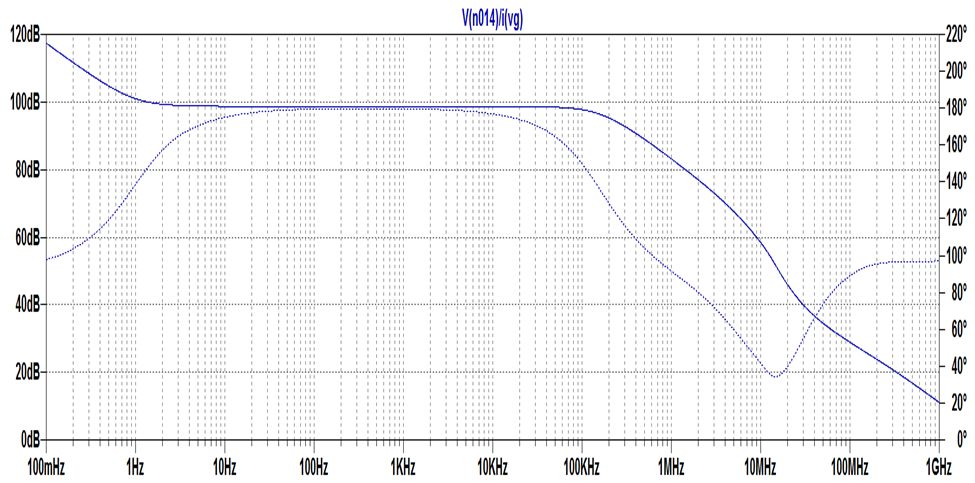
\includegraphics[scale=0.4]{figuras/11-b-Zin.png}
\caption{Impedancia de entrada en función de la frecuencia}
\label{figura11b}
\end{figure}
\begin{center}
Rin(1KHz) = $10^\frac{98,7}{20}K\Omega$ = 86K$\Omega$
\end{center}
Recordemos que el valor calculado fue :\quad Rin=83,9K$\Omega$

\subsubsection{Punto 11.c)}
\textbf{Enunciado : } Medir la impedancia de salida en función de la frecuencia (desde 0,1Hz hasta 1GHz)\\[1cm]
\begin{figure}[H]
\centering
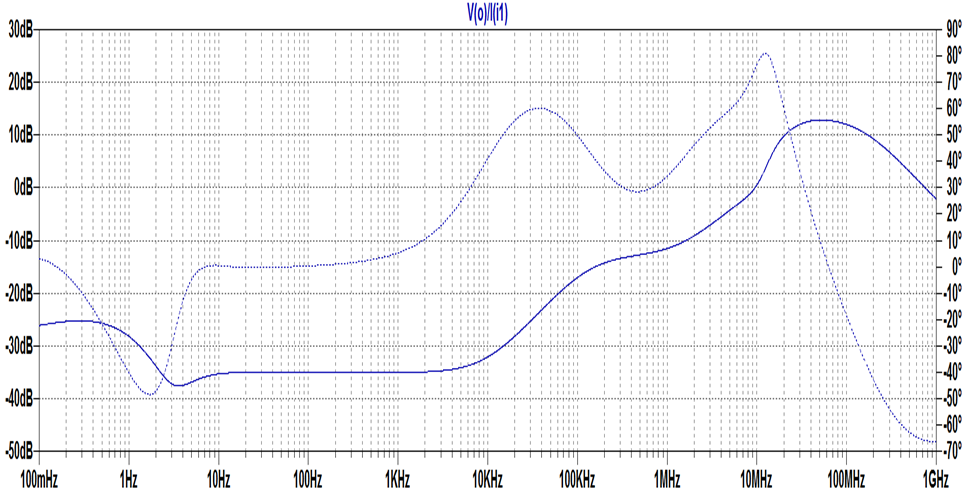
\includegraphics[scale=0.4]{figuras/11-c-Zout.png}
\caption{Impedancia de salida en función de la frecuencia}
\label{figura11c}
\end{figure}
\begin{center}
Ro(1KHz) = $10^\frac{98,7}{20}K\Omega$ = 17,8m$\Omega$
\end{center}
Recordemos que el valor calculado fue :\quad Rin=33,2m$\Omega$

\subsubsection{Punto 11.d)}
\textbf{Enunciado : } Respuesta en frecuencia para 1W sobre la carga)\\[1cm]
Tenemos : $Po=\dfrac{(Vo_{ef})^2}{RL}=\dfrac{(Vop)^2}{2\:RL}=1W$ \quad con Vop=Vo pico\\
Vop = $\sqrt{Po\:\:2\:RL}$ = 4V\quad $\Longrightarrow$\qquad Vip= $\dfrac{Vop}{A}$ = $\dfrac{4V}{28,3}$ = 141mV
\begin{figure}[H]
\centering
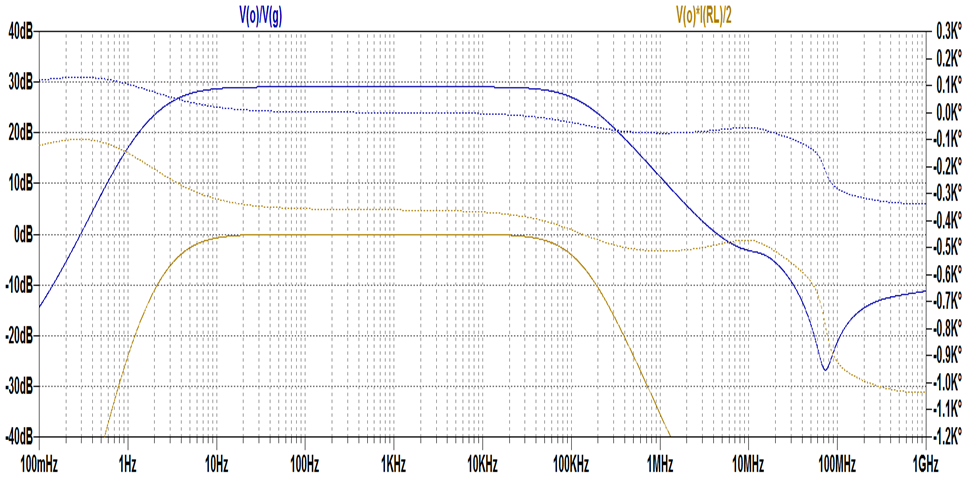
\includegraphics[scale=0.4]{figuras/11-d-Pcarga1W.png}
\caption{Respuesta en frecuencia para 1W sobre la carga}
\label{figura11d}
\end{figure}
\begin{center}
\textcolor{blue}{A(1KHz) = 29dB}\qquad $\Longrightarrow$\qquad A=28,2\\
\textcolor{orange}{Po(1KHz) = 0dB}\qquad $\Longrightarrow$\qquad Po=1W
\end{center}

\subsubsection{Punto 11.e)}
\textbf{Enunciado : } Ancho de banda de potencia\\
Es la máxima frecuencia para la que el amplificador logra reproducir una señal sinusoidal a máxima potencia (hallada en el punto 4 sin deformación)\\[1cm]
Vop = $\sqrt{Po\:\:2\:RL}$ = 21,3V\qquad $\Longrightarrow$\qquad Vip= $\dfrac{Vop}{A}$ = $\dfrac{21,3V}{28,3}$ = 752mV
\begin{figure}[H]
\centering
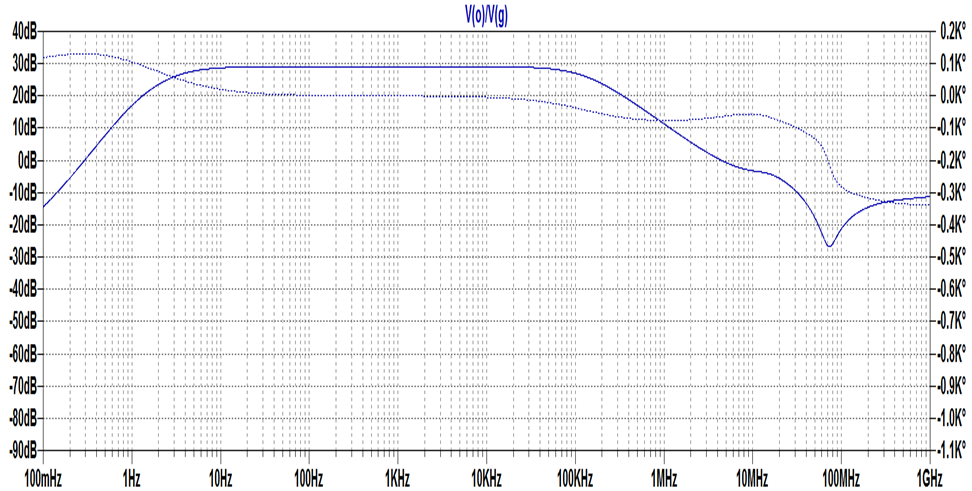
\includegraphics[scale=0.4]{figuras/11-e-BWdePot.png}
\caption{Ancho de banda de potencia}
\label{figura11e}
\end{figure}

\subsubsection{Punto 11.f)}
\textbf{Enunciado : } Respuesta al escalón\\[1cm]
VER COMO HACER SUBSECCIONES PARA ITEMS i, ii, iii, iv

\subsubsection{Punto 11.g)}
\textbf{Enunciado : } Determinar el margen de fase\\[1cm]
A partir de la siguiente figura observamos el margen de fase que le queda a la ganancia de lazo, T, para alcanzar los $180^o$.
\begin{figure}[H]
\centering
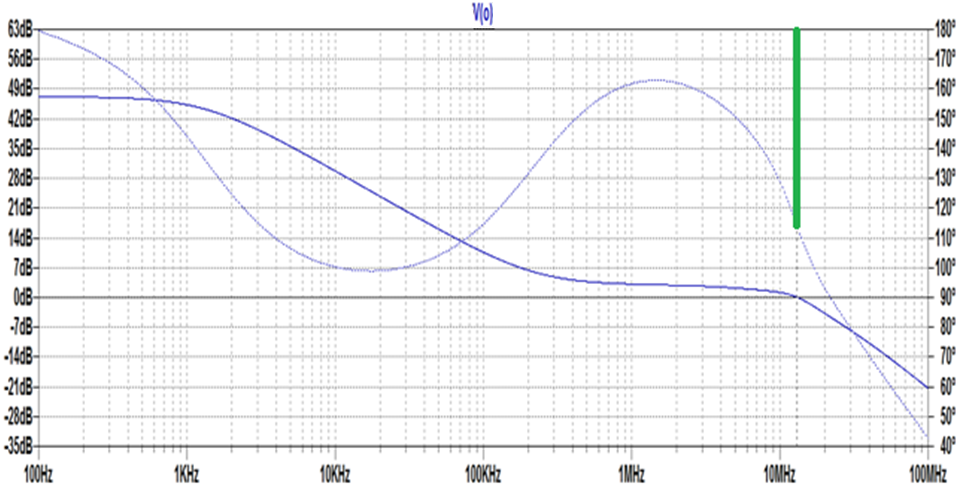
\includegraphics[scale=0.4]{figuras/11-g-margenFase.png}
\caption{Ancho de banda de potencia}
\label{figura11g}
\end{figure}
\begin{center}
Margen de fase :\quad MF $=180^{o}-114^{o}=66^{o}$
\end{center}
\textcolor{red}{VERIFICAR VALOR DE T}

\subsubsection{Punto 11.h)}
\textbf{Enunciado : } Determinar la distorsión armónica a 1KHz y a 10KHz para potencias de 0,1W; 1W; 10W y 90\% de la máxima calculada en el punto 4\\[1cm]
\begin{center}
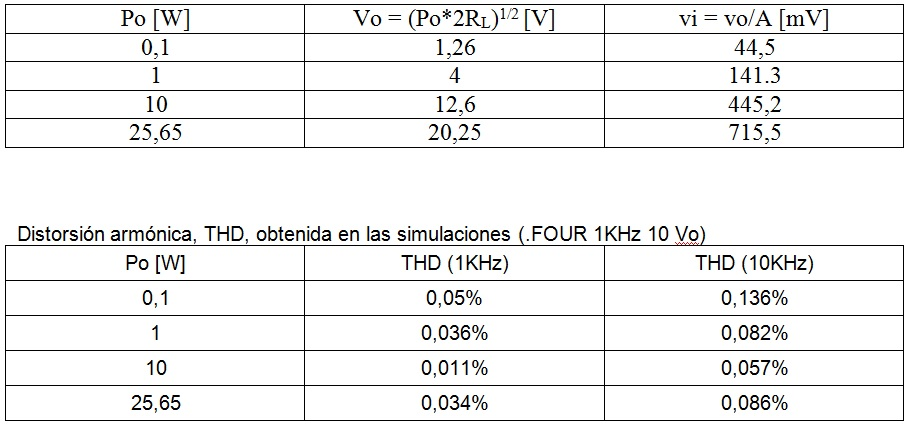
\includegraphics[scale=0.5]{figuras/tabla2.jpg}\\
\end{center}
Vemos que alrededor del 40\% de $Po_{max}$ = 28,5W la distorsión es menor.

\subsubsection{Punto 11.i)}
\textbf{Enunciado : } Determinar la distorsión por intermodulación para potencias de 0,1W; 1W; 10W y 90\% de la máxima calculada en el punto 4\\[1cm]

\subsubsection{Punto 11.j)}
\textbf{Enunciado : } Determinar el Rechazo de Ruido de la Fuente de Alimentación (“PSNR”)\\[1cm]

\end{document}